\chapter{Theory}

\section{Assistive Sports Equipment}

\section{Manufacturing Processes}
Manufacturing is the production of merchandise for use or sale using labour, tools, machine processing or chemical and biological processing. The term is most commonly applied to industrial production, in which raw materials, components or parts are transformed into finished goods that meet a customer's expectations or specifications. \cite{manufacturing} Such finished goods may be sold to costumers for the production of others products who then sell them to end users and consumers.
\par
Manufacturing engineering is the steps through which raw materials are transformed into finished goods. The procedure begins with a part design and material specification. These materials are then modified through manufacturing processes to become the required part.

\subsection{Extrusion}
Extrusion, or extrusion molding is a process used to create objects of a fixed cross-sectional profile. A material is pushed through a die of the desired cross-section, see figure \ref{extrusion}. The two main advantages of this process over other manufacturing processes are its ability to create very complex cross-sections, and to work materials that are brittle, because the material only encounters compressive and shear stresses. Extrusion produces long and thin tubes and tracks with custom profiles, see figue \ref{extrusion_types}. It also forms parts with an excellent surface finish.[1] Metals, plastics and ceramics can be extruded, all under different temperatures and environments. Forms of extrusion include: hot, cold, warm, friction and micro extrusion.

\vspace{0.5cm}
\begin{figure}[htb!]
    \begin{minipage}{.50\textwidth}
    {\setlength{\fboxsep}{0pt}\setlength{\fboxrule}{0.5pt}
    \fbox{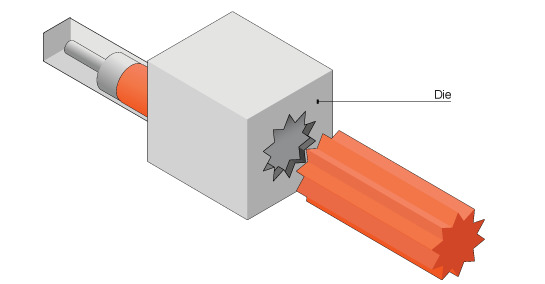
\includegraphics[width=\textwidth]{figures/theory/extrusion.jpg}}}
    \centering
    \captionsetup{justification=centering}
    \caption{Extrusion process}
    \floatfoot{\textit{Source: BBC} \cite{bbc_pictures}}
    \label{extrusion} 
    \end{minipage}
    \hfill
    \centering
    \begin{minipage}{.45\textwidth}
    {\setlength{\fboxsep}{0pt}\setlength{\fboxrule}{0.5pt}
    \fbox{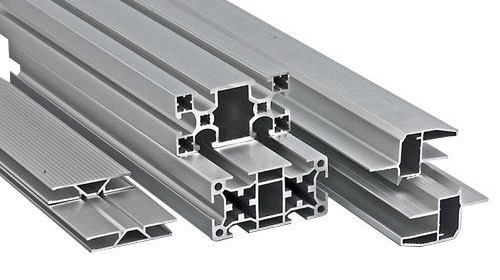
\includegraphics[width=\textwidth]{figures/theory/extrusion_types.jpg}}}
    \centering
    \captionsetup{justification=centering}
    \caption{Extrusion types}
    \floatfoot{\textit{Source: BBC} \cite{bbc_pictures}}
    \label{extrusion_types} 
    \end{minipage}
\end{figure}

\subsubsection{Hot extrusion}
Hot extrusion is a hot working process always performed at temperatures much higher than the recrystallization temperature of the material to be extruded. This is to keep the material from work hardening and making it easier to push through the die. Most hot extrusions are done horizontally on large hydraulic presses that can way up to 12,000 metric tons. Pressures range from 30 to 700 MPa, therefore lubrication is required. For lower temperature extrusions oil or graphite can be used as lubrication. Glass powder is used for higher temperature extrusions. \cite{extrusion2}

\par

\begin{wrapfigure}[]{r}{0.55\textwidth}
    {\setlength{\fboxsep}{0pt}\setlength{\fboxrule}{0.5pt}
    \fbox{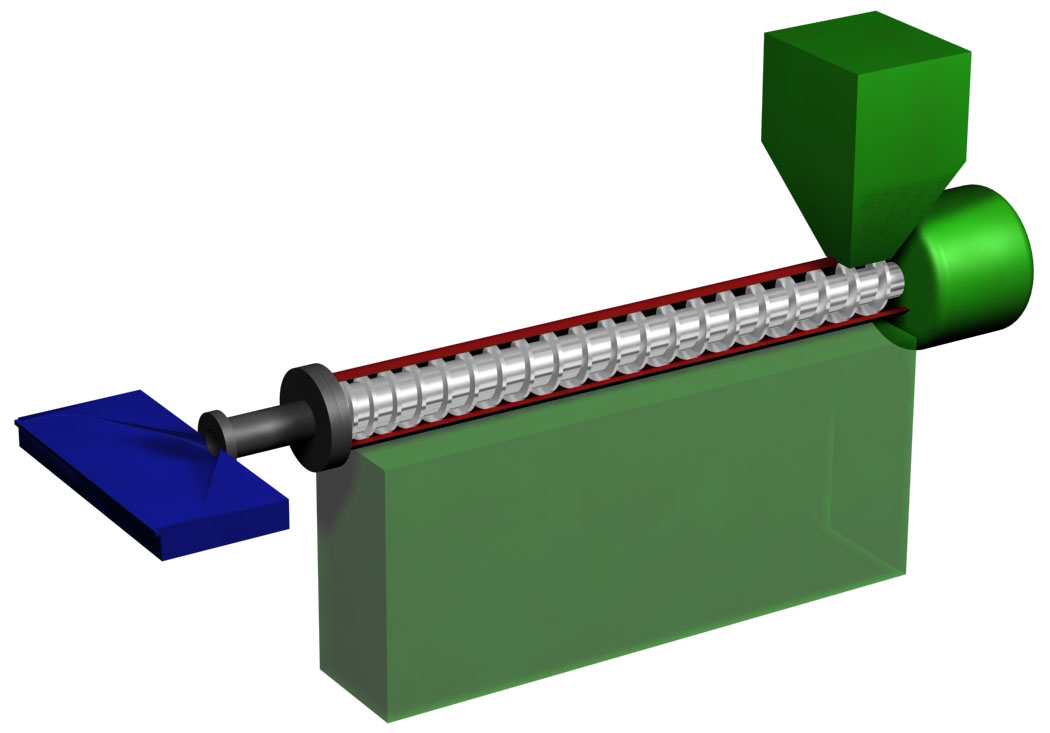
\includegraphics[width=0.55\textwidth]{figures/theory/plastic_extrusion.jpg}}}
    \centering
    \captionsetup{justification=centering}
    \caption{Plastic extrusion process}
    \floatfoot{\textit{Source: Wikimedia} \cite{plastic_extrusion}}
    \label{plastic_extrusion} 
\end{wrapfigure}


Aluminum is the most commonly hot extruded metal, though it can be cold extruded as well. If it is hot extruded it is heated to 300 to 600 °C. Aluminum is commonly extruded to profiles, tubing, tracks, frames, rails, mullions and heat sinks. \cite{aluminum_extrusion} Other commonly hot extruded material include: magnesium, copper, steel, titanium, nickel and other refractory alloys. Plastics are also hot extruded, but under lower temperatures and through a different process, see figure \ref{plastic_extrusion}.


\subsubsection{Cold extrusion}

Cold extrusion is a cold working process usually preformed at ambient temperatures. For most materials this is below the recrystallization temperature. This allows the material to experience work hardening, also known as strain hardening, which strengthens the metal or polymer by plastic deformation. This strengthening is caused by dislocation movements and dislocation generation within the crystal structure of the material. \cite{work_hardening} 
\par
Other advantages for cold extrusion over hot extrusion are the lack of oxidation, closer tolerances, better surface finish, and fast extrusion speeds if the material is subject to hot shortness.\cite{extrusion2} Materials that are commonly cold extruded include: lead, tin, aluminum, copper, zirconium, titanium, molybdenum, beryllium, vanadium, niobium, and steel. 

\subsection{Die Casting}
\begin{wrapfigure}[]{r}{0.65\textwidth}
    {\setlength{\fboxsep}{0pt}\setlength{\fboxrule}{0.5pt}
    \fbox{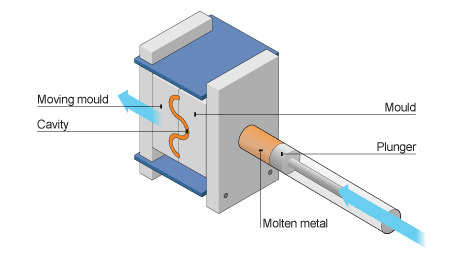
\includegraphics[width=0.65\textwidth]{figures/theory/die_casting.jpg}}}
    \centering
    \captionsetup{justification=centering}
    \caption{Die casting process}
    \floatfoot{\textit{Source: BBC} \cite{bcc}}
    \label{die_casting} 
\end{wrapfigure}
%\vspace{0.5cm}

Die casting is a metal casting process that forces molten metal under high pressure into a mold cavity. The mold cavity is assembled by two hardened steel die/mould half's. The die half's are specially machined into unique hollow shapes and assembled by a high pressure clamping unit. One of the dies are stationary and equip with an injection tube. Molten metal is plunged through the injection tube at pressure up to 138 MPa and fill the cavity, see figure \ref{die_casting}. After the molten metal is injected into the dies, it rapidly cools and solidifies into the final part, called the casting. The cooling time can be estimated from several thermodynamic properties of the metal, the maximum wall thickness of the casting, and the complexity of the die. \cite{die_casting} Once solidified the casting can be ejected and trimmed of excess material. 
\par
Most die castings are made from non-ferrous metals such as aluminum, magnesium or zinc. Depending on the type of metal being cast, a hot- or cold-chamber machine is used. Hot chamber machines are used for alloys with low melting temperatures, such as zinc, tin, and lead. Having low melting temperatures allow these alloys to be heated and pumped through the die to the cavity. The temperatures required to melt other alloys with high melting temperatures such as aluminum, brass and magnesium would damage the pumping system. Hence, the molten metal is kept separate from the die casting machine and plunge into the cavity. \cite{die_casting2}  
\par
Die casting is an accurate manufacturing process and is therefore commonly used to produce geometrically complex metal parts. Often, if a part is too complex to be extruded it is cast. The two process are very similar as they both require an initial investment for the die's and tooling equipment and offer a cheap and repeatable production of custom parts. Other significant advantages over other manufacturing processes are cost savings part price and overall production, variable wall thickness, tighter tolerances, ability to combine multiple parts, fast production, less material scarp and long tool life.

\subsection{Milling}

\cite{cnc_picture}
\subsection{Laser cut and bending, sheet metal}

\subsection{Injection moulding}

\subsubsection{Silicone mould PUR}

\subsubsection{XXX}

\subsection{Vacuum casting}

\subsection{Finish and coating}

\subsection{Textile}

Details
Materials
Use cases, 
Advantages






%\subsection{Metal}
%A metal is a material (an element, compound, or alloy) that is typically hard when in solid state. Metals are generally malleable—that is, they can be hammered or pressed permanently out of shape—as well as fusible (melted, welded) and ductile (thinned, bent, handled). \cite{metal}


\section{Manufacturing Locations}



\section{Product Development}

\subsection{Methodologies}

\subsubsection{IPM model}

\subsubsection{Stage Gate Model}

\subsubsection{Set-Based Design}

\subsubsection{NBD - Nature of Market}

\subsubsection{MVP - Minimum Viable Product}
Minimum Viable Product (MVP), is one of the most important lean start-up techniques. An MVP is a product with just enough features to satisfy early customers, and to provide feedback for future product development. Developers can deploy this product to a potential user as an early adopter. Giving a user a functional product with less features gives more power to the user to give feedback on what is missing. If a company is in a constant reworking prototyping stage, this strategy lowers the cost, maximizes the information and avoids building products that customers do not want. The final, complete set of features is only designed and developed after considering feedback from the product's initial users.



\subsection{Prototyping}

\subsubsection{What is prototyping}

\subsubsection{Experience prototyping}

Experience prototyping engages the designers, clients and users with the prototypes. This helps the designer understand, explore or communicate what it is like to engage with the product. According to Buchenau and Suri 2000, Experience Prototyping is particularly powerful in three activities within prototyping, see list below.

\vspace{0.5cm}
\begin{enumerate}
    \item Understanding existing user experiences and context
    \item Exploring and evaluating design ideas
    \item Communicating ideas to an audience
\end{enumerate}
\vspace{0.5cm}

Experience Prototyping is essentially a cheap and effective way to assess various parts of design or technical solution during the product development.\cite{christer}